%\section{\centering Experimental Setup}
\chapter{Object Reconstruction}
%\chapter*{\centering Experimental Setup}
\label{ch:ObjReco}

The CMS detector attempts to identify all particles produced in $pp$ collisions. However, all of the data from an event is provided as hit patterns in the subdetectors and to simplify the analysis of these hit patterns they are first converted into physics objects. This chapter will describe the process of reconstructing physics objects from the information provided by the CMS detector.

%the Particle Flow algorithm used by CMS to reconstruct all stable particles: electrons, muons, photon, charged and neutral hadrons. 

\section{The Particle Flow Algorithm}

The Particle Flow (PF) algorithm~\cite{PFAlgorithm, PFReconstruction} optimally combines information from all of the subdetectors to identify and reconstruct every individual particle produced in a proton-proton (pp) collision. To accomplish this, the CMS detector was designed with a nearly fully efficient tracking system to precisely reconstruct tracks and vertices and a calorimeter with excellent granularity to disentangle overlapping showers. The PF algorithm is comprised of three main elements: iterative tracking, calorimeter clustering, and the link algorithm.

\subsection{Iterative Tracking}

To reconstruct the charged particles from a $pp$ collision, the hits in the tracker need to be converted into a collection of tracks. The tracking software used by the PF algorithm is called the Combinatorial Track Finder (CFT)~\cite{TrackReco} and it allows pattern recognition and track fitting to occur in the same framework. The CFT is run six times with the reconstruction criteria loosening for each iteration to achieve both a high efficiency and low fake rate. Each iteration is comprised of four steps: seed generation, track finding, track fitting, and track selection.

Seed generation determines initial track trajectories from the minimum number of hits necessary to define a trajectory in a magnetic field. Five parameters are needed to define a helical trajectory and thus, either 3 hits or 2 hits and an additional constraint that the particle originates from the beam spot are used to define the seeds. These seeds are required to pass some minimum $p_{T}$ threshold and must be consistent with originating from the $pp$ interaction region. Next, the initial track trajectories are extrapolated out and at each detector layer the hit with the position that produces the smallest $\chi^{2}$ to the extrapolated trajectory is added to the track. This process is repeated at each detector layer until the end of the tracker is reached. When there is no hit along the trajectory at a certain layer, a ``ghost'' hit is added to the track. Tracks are discarded after a certain number of ghost hits are recorded. To obtain the full information of the trajectory, tracks are refitted with all hits using a Kalman filter and smoother~\cite{KalmanFilter}. Finally, tracks are selected if they pass a certain number of quality requirements such as the number of layers with hits, the $\chi^{2}/\mathrm{ndf}$ of the track fit, and the compatibility that the track originates from the primary vertex. This greatly reduces the number of fake tracks. 

%To define a trajectory in a magnetic field, five parameters are needed and thus seed generation uses 3 hits in the tracker or 2 hits in the tracker and an additional constraint that the particle originates from the beam spot to define initial trajectories. 

%These seeds are required to pass some minimum $p_{T}$ threshold and must be consistent with originating from the proton-proton interaction region. Next, the initial track trajectories are extrapolated out and at each detector layer the hit with the smallest $\chi^{2}$ to the trajectory is added to the track. This process is repeated at each detector layer until the end of the tracker is reached. When there is no hit along the trajectory at a certain layer a “ghost” hit is added to the track. Tracks are discarded after a certain amount of ghost hits are recorded. To obtain the full information of the trajectory, tracks are refitted with all hits using a Kalman filter and smoother~\cite{KalmanFilter}. Finally, tracks are selected if they pass a certain amount of quality requirements such as the number of layers with hits, the $\chi^{2}/ndf$ of the track fit, and the compatibility that they originate from the primary vertex. This greatly reduces the number of fake tracks. 

\subsection{Calorimeter Clustering}

There are four purposes to the clustering algorithm in the calorimeter: detect and measure the energy and direction of neutral particles, separate these neutral particles from energy deposits of charged ones, reconstruct and identify electrons and all accompanying Bremsstrahlung photons, and assist the energy measurement of charged hadrons when track parameters are not accurately determined. The clustering algorithm is therefore designed for a high detection efficiency for low-energy particles and a separation of close energy deposits from the high granularity calorimeter. Clustering is performed separately in each subdetector as follows.

First, the seed for a cluster of nearby hits is identified as the hit with the maximum energy that is above a given threshold. Topological clusters are then created by adding cells that are adjacent to the cells already in the cluster and have an energy above a given threshold. Finally, the final energy and position of the clusters is determined through an iterative expectation-maximization algorithm. 

\subsection{The Link Algorithm}

The purpose of the link algorithm is to connect the different PF elements from the subdetectors to fully reconstruct a particle. The elements that can be linked are charged-particle tracks, calorimeter clusters, and muon tracks. The link algorithm creates blocks of elements which contain two or three elements. 

A link between a track and a calorimeter cluster is made if the extrapolated track from the tracker lands within the cluster. Clusters from different calorimeter subdetectors are linked when the position in the more granular calorimeter is within the cluster envelope in the less granular calorimeter. And finally, links between tracker tracks and muon tracks are made when a global fit of the combied tracks returns an acceptable $\chi^{2}$. 

\subsection{Particle Identification}

Each block of elements is identified as specific particles in the following way. First, muons are identified when the momentum of the combined tracks in the tracker and muon detector is within $3 \sigma$ of the tracker momentum. The corresponding tracks are then removed from the block. Secondly, electrons are identified by finding tracks that fit the criteria of an electron track: short tracks that lose energy from Bremsstrahlung. These tracks are refit with a Gaussian-Sum fitter~\cite{GausSumFilter} to project their trajectories out to the ECAL and find an intersecting cluster. The corresponding track and ECAL cluster are then removed from the block. Thirdly, charged hadrons are identified from the remaining tracks and are associated to clusters in the HCAL if the cluster energy falls within the uncertainties of the track momentum. Finally, the remaining clusters in the HCAL and ECAL are associated with neutral hadrons and photons, respectively. 

\section{Vertex Reconstruction}

Vertex reconstruction locates all of the $pp$ interactions within an event so that they can be classified. The \textit{primary} vertex results in high $p_{T}$ particles and is of most interest because the primary signature of the event originates from it. The remaining vertices are referred to as \textit{pileup} and most of these interactions produce soft particles that contribute to the overall hadronic activity within an event, and can obscure the interesting processes. In 2016, the CMS detector recorded between 45 to 60 pileup vertices for each event and therefore determining the activity from pileup is crucial for analyses.

%The purpose of vertex reconstruction is to measure the location of all proton-proton interactions within an event. 
Vertex reconstruction consists of three steps: track selection, clustering tracks originating from the same vertex, and fitting the tracks for the position of each vertex. Track are selected that are produced promptly in the primary interaction region. This is done by placing requirements on the impact parameter off the track relative to the center of the beam, the number of hits within the track, and the $\chi^{2}$ of the fit trajectory. The tracks are then clustered according to their z-coordinate at their point of closest approach to the center of the beam spot. Finally, the position of each vertex is determined by fitting each cluster of tracks~\cite{TrackReco}. 

\section{Jet Reconstruction}
\label{sec:jetReco}
In an attempt to reconstruct the hadronization of a quark or gluon, the hadrons and non-isolated leptons of an event are clustered together to form jets. In this analysis, the ``anti-$k_{t}$'' algorithm is used to create jets. This algorithm iteratively clusters particles together by defining two distance parameters
%distance between particles $i$ and $j$ as

\begin{equation}
d_{ij}=min(k_{ti}^{2p},k_{tj}^{2p})\frac{\Delta_{ij}^{2}}{R^{2}},
\end{equation}
\begin{equation}
d_{iB} = k_{ti}^{2p},
\end{equation}
where $k_{ti}$ is the transverse momentum of particle $i$, $\Delta_{ij}^{2} = (y_{i}-y_{j})^{2}+(\phi_{i}-\phi_{j})^{2}$, $y_{i}$ is the rapidity, $\phi_{i}$ is the azimuth, R is the chosen cone radius, and $p=-1$ gives the anti-$k_{t}$ algorithm. The distance between particles $i$ and $j$, $d_{ij}$, is compared to $d_{iB}$, the distance between particle $i$ and the beam. If $d_{ij}$ is smaller than $d_{iB}$ then $i$ and $j$ are recombined, but if $d_{ij}$ is larger then $i$ is called a jet and removed from the remaining particles. This continues until are particles have been clustered into jets.

The anti-$k_{t}$ algorithm clusters soft particles to hard ones, so that a jet's axis is mainly defined by its hard constituents. This is a key feature of the algorithm because the jet's axis will not dramatically change when soft radiation from pileup is removed from the event. When two hard particles are nearby, they are either clustered together or the soft particles are shared between them based on the size of the cones being reconstructed. 

\section{Missing Transverse Energy}

The initial momentum of the colliding constituents in the protons at CMS is unknown, however it is known that their transverse momentum is zero. Therefore, by conservation of momentum, the combined transverse momentum of all of the particles produced in the collision is zero. However, weakly interacting particles, such as neutrinos, can avoid detection and cause there to be an imbalance in the transverse momentum of a collision. These signatures are predicted by many theoretical models and therefore, a useful quantity in the analysis of CMS data is the missing transverse momentum

\begin{equation}
\vec{\cancel{E}_{T}}= -\sum_{detected\;particles} \vec{p_{T}}.
\end{equation}
This quantity is referred to as MET throughout this paper.

\section{$b$-tagging}

The identification of jets arising from the hadronization of $b$ quarks is crucial for searches for new physics and for measurements of standard model processes. These jets can be distinguished from jets initiated by gluons or light flavor quarks due to the long lifetime of B hadrons, about 1.5 ps, which causes the B hadron to decay within the jet and form a secondary vertex. These secondary vertices are displaced hundreds of micrometers away from the primary vertex and therefore, the high resolution of the pixel detector is the leading reason $b$ quarks are identified efficiently.

CMS employs several b tagging algorithms~\cite{BTagging}, although the combined secondary vertex (CSVv2) algorithm is primarily used. The CSV algorithm uses secondary vertices, which are reconstructed from the tracks of charged particles within a jet, and track impact parameters, which are the points of closest approach from each track to the primary vertex, as input to a likelihood based discriminant. The shape of the CSVv2 discriminant is shown in Figure~\ref{fig:CSV}.

\begin{figure}[h!]
\begin{center}
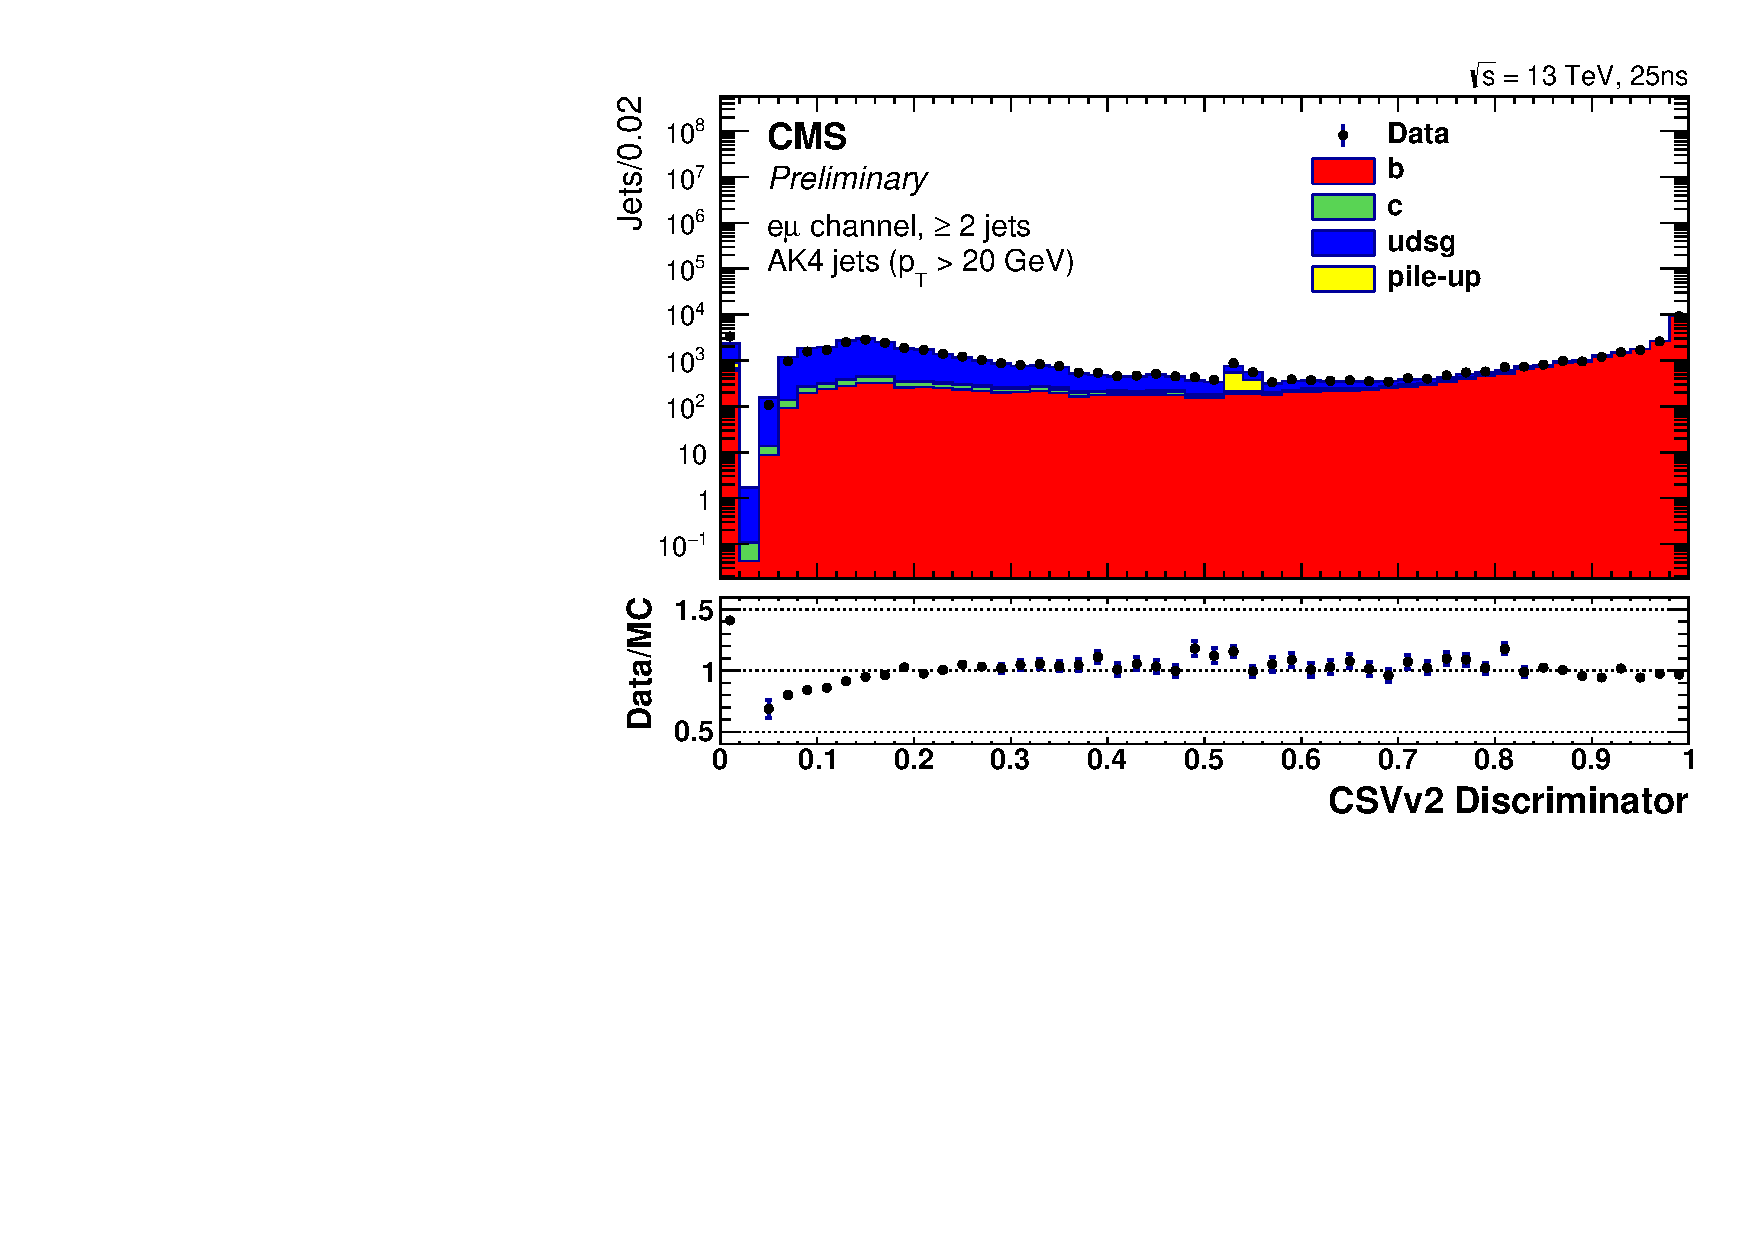
\includegraphics[width=3.5 in]{ObjectReconstruction/CMS-PAS-BTV-15-001_Figure_003-f.pdf}
\end{center}
\caption{Discriminator values for the combined secondary vertex (CSVv2) algorithm in a dilepton $t\bar{t}$ topology. The total number of entries in the simulation is normalized to the observed number of entries in data. The small bump between discriminator values of 0.5 and 0.6 are due to tracks or jets from pileup collisions~\cite{BTagging}.}
\label{fig:CSV}
\end{figure}


\section{Double $b$-tagging}

A more challenging tagging technique is the identification of jets that contain two $b$ quarks. This is especially important for the analysis presented in this thesis, where a Higgs decaying to $\mathrm{b\bar{b}}$ is reconstructed within a single large cone jet, also referred to as a \textit{fatjet}. In Run I of the LHC, two different techniques were used to identify jets containing two $b$ quarks: fatjet $b$ tagging and subjet $b$ tagging. Fatjet $b$ tagging applies the standard $b$ tagging algorithm to a fatjet but with the track and vertex criteria relaxed due to the larger jet cone size. Subjet $b$ tagging defines two subjets within the fatjet and then individually $b$ tags each of these. These two approaches complimented each other to an extent. Fatjet $b$ tagging performs better in the high tagging efficiency regime where the presence of displaced tracks improves the performance, while subjet $b$ tagging performs better in the high purity regime where it can rely on the reconstruction of two distinct secondary vertices. For jets with higher $p_{T}$, the subjets begin to overlap and subjet $b$ tagging becomes inefficient due to the double counting of tracks. A diagram of these two approaches can be seen in Figure~\ref{fig:2btagging} and due to the complentary nature of these techniques it is clear that there is a possibility for improvement with a more efficient tagger. 

\begin{figure}[h!]
\begin{center}
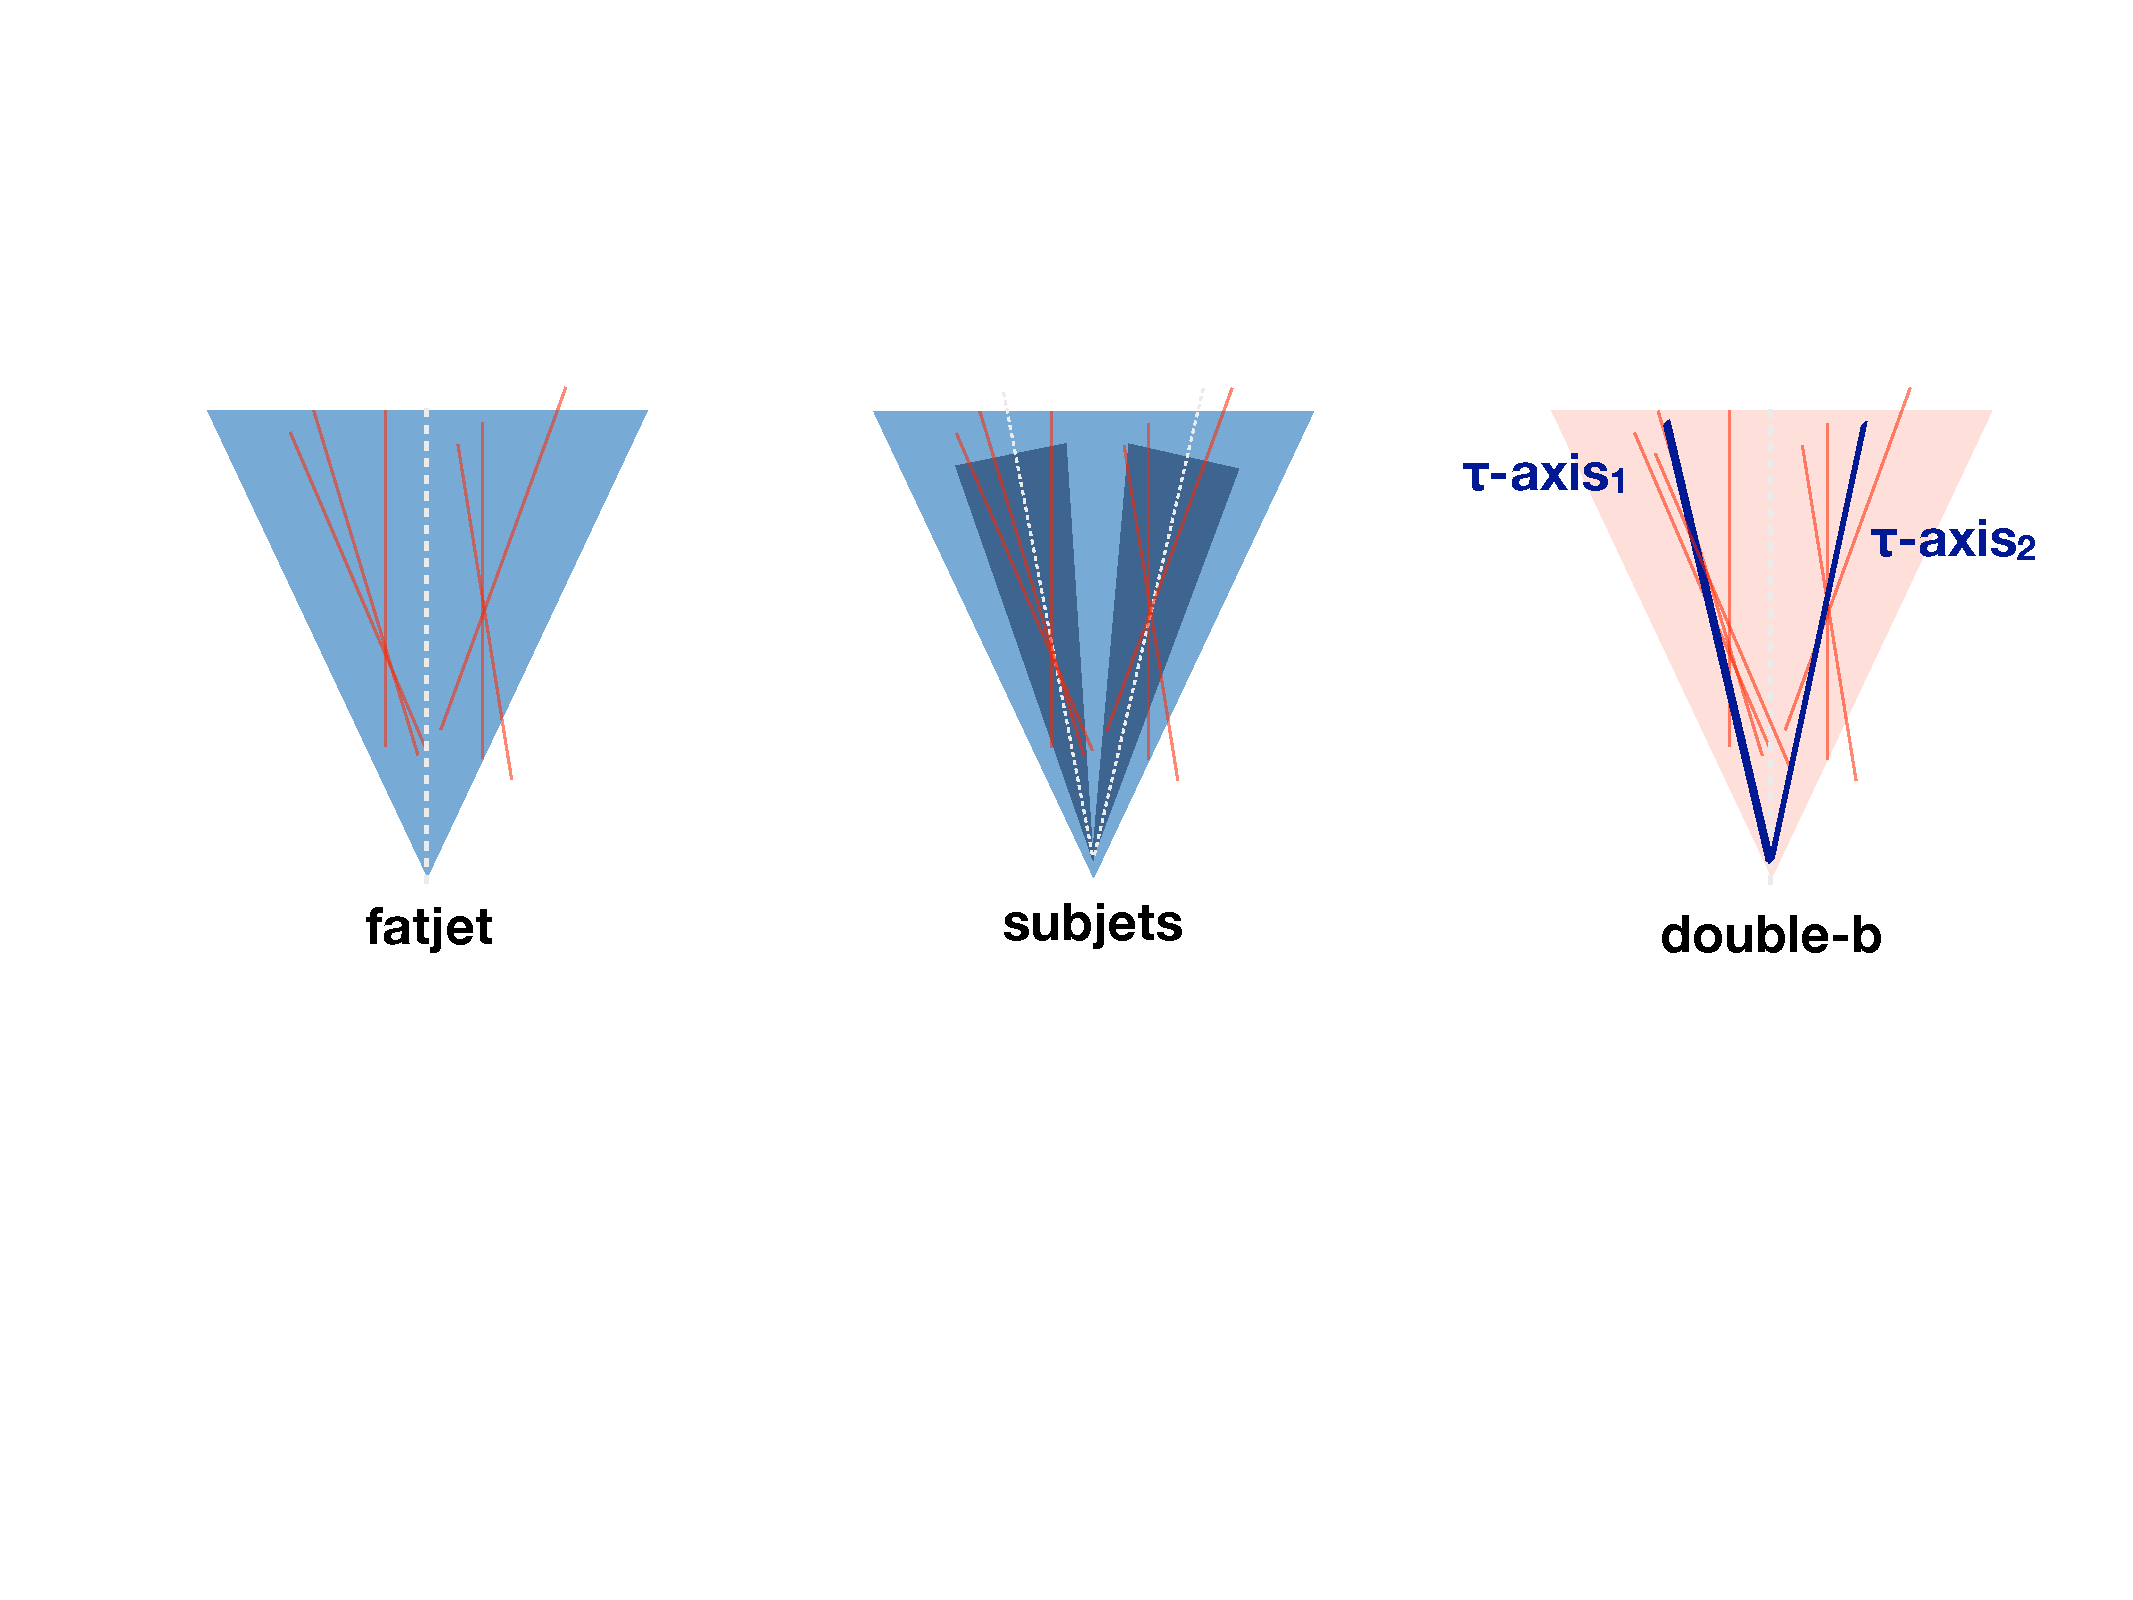
\includegraphics[width=4.5 in]{ObjectReconstruction/CMS-PAS-BTV-15-002_Figure_001.pdf}
\end{center}
\caption{Schematic comparison of the fatjet and subjet b tagging approaches and the double-b tagger~\cite{DoubleB}.}
\label{fig:2btagging}
\end{figure}

Therefore, a dedicated multivariate algorithm, called the ``double-b tagger,'' was developed to holistically tag jets containing two $b$ quarks. The double-b tagger reconstructs secondary vertices within the fatjet independently of the jet clustering and then associates each secondary vertex to a subjet axis in order to reconstruct the decay chains of the two B hadrons. At the same signal efficiency, the mistag rate of the double-b tagger is lower by about a factor of 2 compared to the previous tagging approaches, as shown in Figure~\ref{fig:DoubleBperformance}. 

\begin{figure}[h!]
\begin{center}
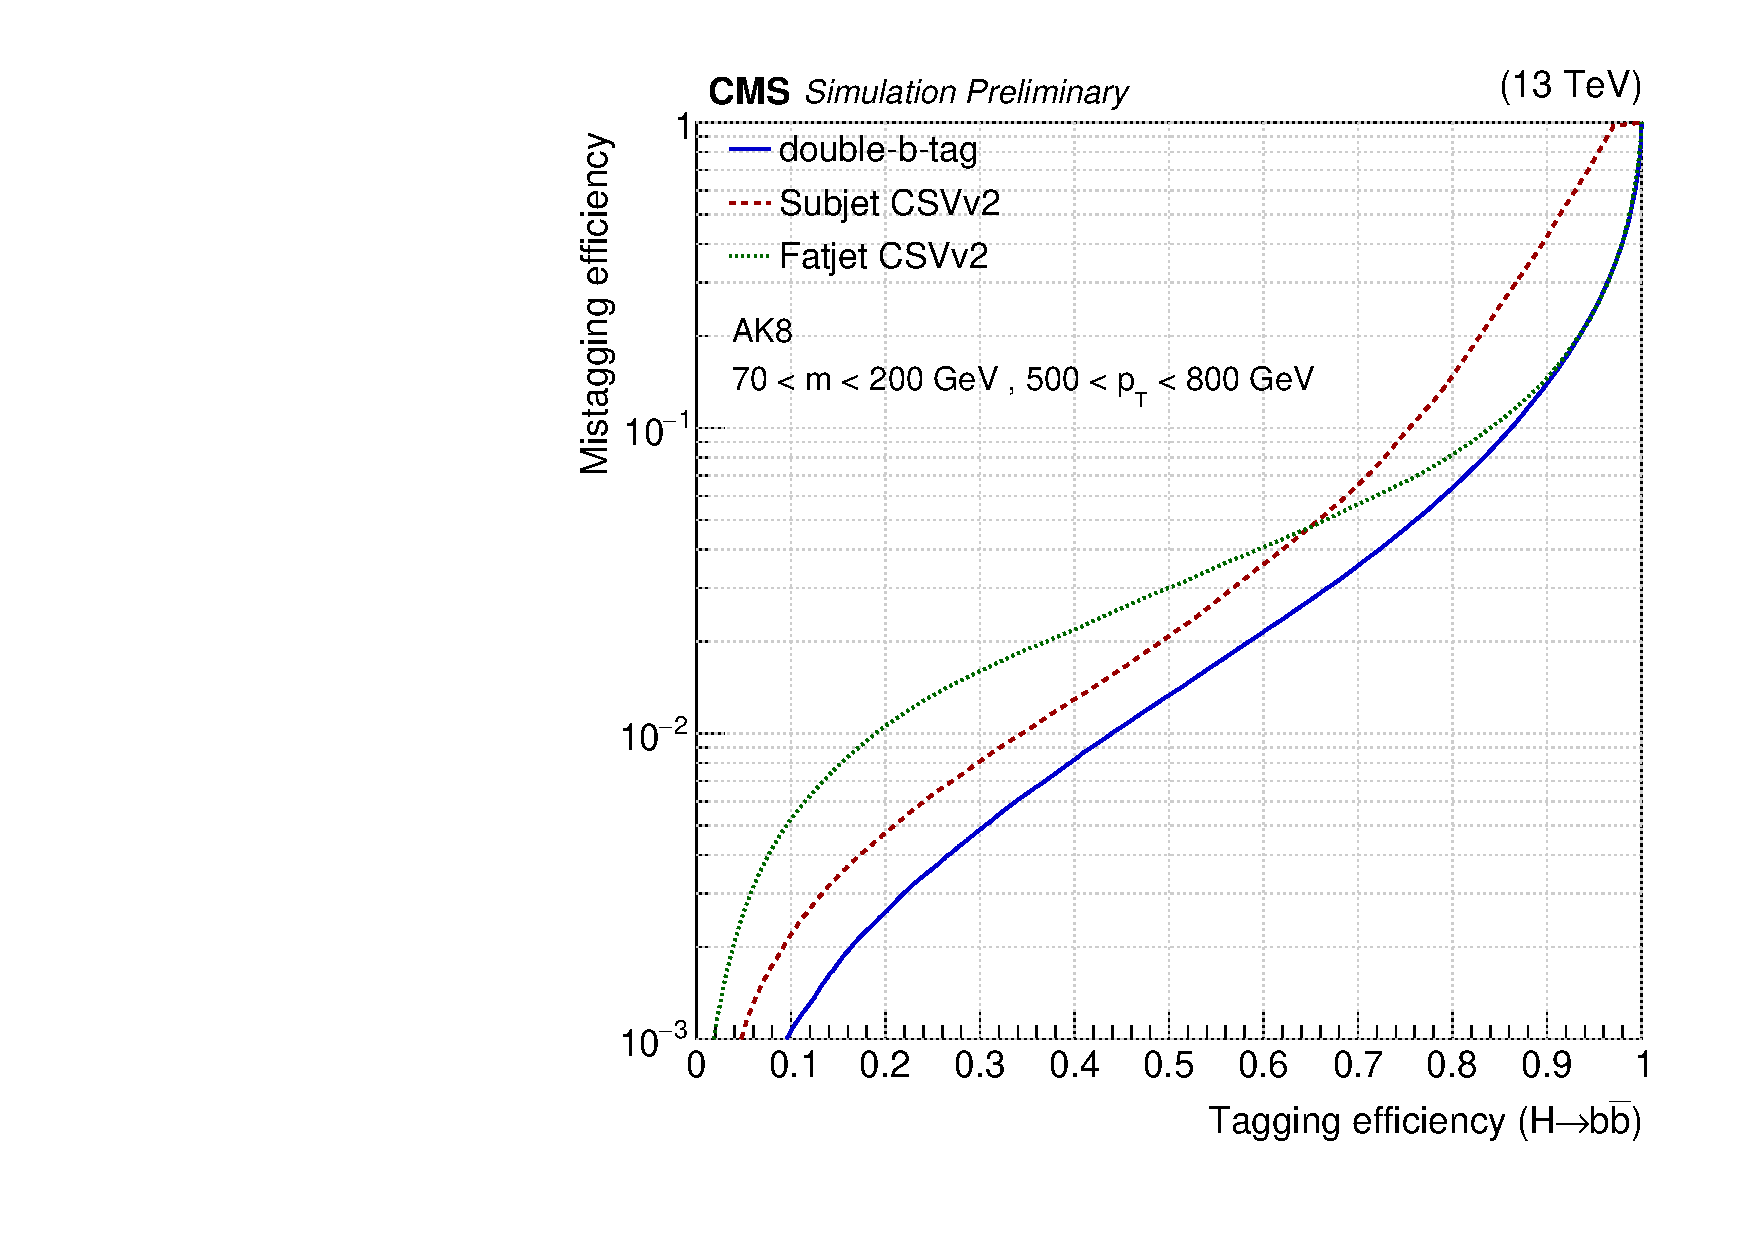
\includegraphics[width=4 in]{ObjectReconstruction/CMS-PAS-BTV-15-002_Figure_003-b.pdf}
\end{center}
\caption{Comparison of the performance of the double-b tagger, the CSVv2 subjet $b$ tagging, and fatjet $b$ tagging using the CSVv2 algorithm for $500 < p_{T} < 800$ GeV jets. The tagging efficiency for signal is evaluated using boosted $\mathrm{H}\rightarrow\mathrm{b\bar{b}}$ jets from simulation. The mistag rate is evaluated for simulated QCD jets containing zero, one or two $b$ quarks\cite{DoubleB}.}
\label{fig:DoubleBperformance}
\end{figure}












